\documentclass[../main.tex]{subfiles}

\begin{document}
\section{Theory} \label{sec:theory}
\subsection{Wavefunction of Helium} \label{sec:QMProb}
The single-particle wave function of an electron $i$ in the $1s$ state is given in terms of a dimensionless variable (the wave function is not normalized) as

\[\psi_{1s}(\mathbf{r}_i) = e^{-\alpha r_i}\]
where the electron position $\mathbf{r}_i$ is
\[\mathbf{r}_i = x_i \mathbf{e}_x + y_i \mathbf{e}_y + z_i \mathbf{e}_z\]
and its distance from the origin $r_i$ is
\[r_i = \sqrt{x_i^2 + y_i^2 + z_i^2}\]

$\alpha$ is a parameter set to 2, which corresponds to the carge of the Helium atom, $Z = 2$. \cite{Hjorth-Jensen2019}


For our system with two electrons, we have the product of the two $1s$ wave functions defined as
\[\Psi(\mathbf{r}_1, \mathbf{r}_2) = e^{-\alpha(r_1 + r_2)}\]

This leads to the integral which will be solved nummerically with the  different methods mentioned earlier.
The value of the integral corresponds to the expectation value of the  energy between the two electrons repelling each other due to Columb interactions.

\begin{equation}
  \langle \frac{1}{|\mathbf{r}_1 - \mathbf{r}_2|} \rangle = \int_{\infty}^\infty d\mathbf{r}_1 d\mathbf{r}_2 e^{-2\alpha(r_1 + r_2)} \frac{1}{|\mathbf{r}_1 - \mathbf{r}_2|}
  \label{eq:int-to-solve}
\end{equation}
\vspace{1cm}

This is the integration that will be performed numerically in multiple ways in this paper. The analytical result is $5\pi^2/16^2 \approx 0.1927657$.

\subsection{Gaussian Quadrature} \label{sec:GQ}
The main idea of the Gaussian quadrature is to integrate over a set of points $x_i$ not equally spaced with weights $w_i$. The weights are found through orthogonal polynomials(Laguerre and Legendre polynomials) in a set interval. The points $x_i$ are chosen in a optimal sense and lie in the interval.

The intgral is approximated as
\[\int_a^b W(x)f(x) \approx \sum_{i=1}^n \omega_i f(x_i) \]

For a more detalied derivation and explanation of Gaussian quadrature see \cite{MortenMC2019}. The program used to find mesh points and weights is found at \href{https://github.com/kmaasrud/Project-3/blob/master/code/Gauss-Quadrature/src/gauleg.cpp}{\texttt{/code/Gauss- Quadrature/src/gauleg.cpp
}}.

\subsubsection{Gauss-Legendre}\label{sec:GLQ}
Using Gauss-Legendre quadrature with Legendre polynomials will make it possible to solve the integral numerically. The first step is to change the integration limits from  $-\infty$ and $\infty$ to $-\lambda$ and $\lambda$. The $\lambda$'s are found by inserting it for $r_i$ in the expression $e^{-\alpha r_i}$ because $r_i \approx \lambda$ when $e^{-\alpha r_i} \approx 0$. From figure \ref{fig:plot}, $\lambda \in [-5,5]$ is therefore a good approximation for the integration limits.

\begin{figure}[!h]
  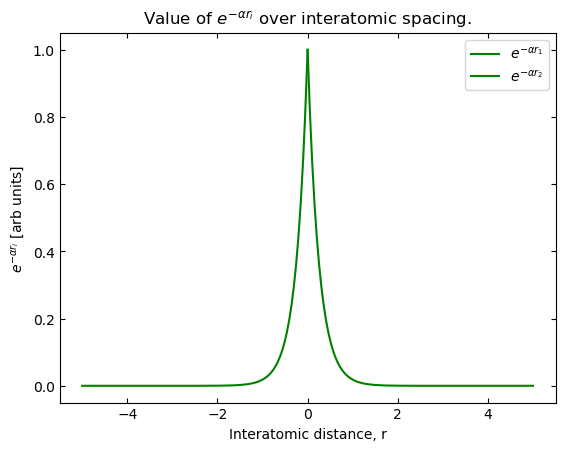
\includegraphics[width=\textwidth]{img/expfunc_plot.png}
  \caption{Plot of wavefunction in one dimension}
  \label{fig:plot}
\end{figure}
\FloatBarrier


Eventually we end up with a sixdimensional integral, where all six integration limits are the same.

\[\int_a^b\int_a^b\int_a^b\int_a^b\int_a^b\int_a^b e^{-x}f(x)dx \approx \sum_{i=1}^n w_i f(x_i)\]

\subsubsection{Improved Gauss-Quadrature: Laguerre} \label{sec:improved_GQ}
The Gauss-Legendre quadrature gets the job done, but it takes a large number of integration points to yield satisfactory results, and the choise of $\lambda$ is very hard to make. By changing to spherical coordinates and replacing Legendre- with Laguerre polynomials an improvement in accuracy is expected. The Laguerre polynomials are defined for  $x \in [0, \infty)$, and in spherical coordinates:
\\

\begin{equation}
  d\mathbf{r}_1 d\mathbf{r}_2 = r_1^2 dr_1 r_2^2 dr_2 dcos(\theta_1) dcos(\theta_2) d\phi_1 d\phi_2
  \label{eq:sphere-cord1}
\end{equation}
\\
with

\begin{equation}
  \frac{1}{r_{12}} = \frac{1}{\sqrt{r_1^2 + r_2^2 - 2r_1r_2cos(\beta)}}
  \label{eq:sphere-cord2}
\end{equation}
\\and

\begin{equation}
  cos(\beta) = cos(\theta_1)cos(\theta_2) + sin(\theta_1)sin(\theta_2)cos(\phi_1 - \phi_2)
  \label{eq:sphere-cord3}
\end{equation}
\\

For numerical integration, the deployment of the following relation is nessecary:

\[\int_0^\infty e^{-x}f(x)dx \approx \sum_{i=1}^n w_i f(x_i)\]
where $x_i$ is the $i$-th root of the Laguerre polynomial $L_n(x)$ and the weight $w_i$ is given by
\\
\[w_i = \frac{x_i}{(n+1)^2 [L_{n+1}(x_i)]^2}\]
\\
The Laguerre polynomials are defined by Rodrigues formula:
\[L_n(x) = \frac{e^x}{n!}\frac{d^n}{dx^n}\left(e^{-x} x^n\right) = \frac{1}{n!}\left(\frac{d}{dx}-1\right)^n x^n\]
or the recursive relation:
\begin{align*}
  L_0(x) &= 1\\
  L_1(x) &= 1 - x\\
  L_{n+1}(x) &= \frac{(2n + 1 - x)L_n(x) - nL_{n-1}(x)}{n+1}\\
\end{align*}
<<<<<<< HEAD

=======
>>>>>>> 75b00ec75b46f7edda1c003b96e40a4c94604c4a


\subsection{Monte Carlo}
\subsubsection{Generalized}
\label{sec:MC}
Monte Carlo integration is based on the idea of finding the mean of a function in a domain by sampling random function values. This mean multiplied by the volume of the domain will be an approximation of the integral. \\

Say we have an integral $I$ of $f(\mathbf x)$ we want to find:

\begin{equation*}
  I=\int_D f(\mathbf x)d\mathbf x
\end{equation*}
where $\mathbf{x}$ is in the domain $D$. This integral can be approximated by using random numbers distributed on $D$ by the probability distribution function (PDF) $p(\mathbf x)$. Discretizing, the approximated integral now becomes

\begin{equation}
  I \approx \langle I \rangle = \frac{1}{N}\sum_{i=0}^N\frac{f(\mathbf x_i)}{p(\mathbf x_i)},
  \label{eq:genapproxMC}
\end{equation}
where  $N$ is the number of sampled values.

% ---------------------------------------------------------------
\subsubsection{Naïve approach (uniform PDF)} \label{sec:naiveMC}
To solve our six-dimensional integral, we first take the naïve approach and distribute our randomly chosen variables on the uniform distribution

\begin{equation*}
  \theta (x) = \bigg\{ \begin{matrix}\frac{1}{b-a}, & \text{for}\ x\in[a,b] \\ 0 & \text{else}\end{matrix},
\end{equation*}
and keep our variables $\mathbf r_1$ and $\mathbf r_2$ in cartesian coordinates. Putting the uniform distribution into (\ref{eq:genapproxMC}), we get the naïve approximation of an integral:

\begin{equation}
  \langle I\rangle = \frac{V}{N}\sum_{i=0}^Nf(\mathbf x_i).
\end{equation}

Here $V$ is the integration volume (for $d$ dimensions in cartesian coordinates $V=(b-a)^d$, with $b$ and $a$ being the integration limits for each dimension). Going back to our original integral (\ref{eq:int-to-solve}), our approximation of it using this method is

\begin{equation}
  \langle I \rangle = \frac{(b-a)^2}{N}\sum_{i=0}^Ne^{-2\alpha(r_{1,i}+r_{2,i})}\frac{1}{|\mathbf r_{1,i}-\mathbf r_{2,i}|},
  \label{eq:naive-approx}
\end{equation}
with $\mathbf r_{1/2,i}$ being randomly chosen vectors and $b=a=\infty$, or our approximation of infinity, namely $\lambda = 5$ (see section \ref{sec:GLQ}).

% ------------------------------------------------------------------------------------
\subsubsection{Importance sampling (exponential distribution)} \label{sec:improvedMC}

As mentioned in section \ref{sec:GLQ}, our integrand quickly goes to zero. This means that inserting bigger approximations for infinity, $\lambda$, requires a greater number of sampling points, since we are not sure if the random numbers will give us the significant values of the integrand.

A sensible way around this is to distribute the randomly chosen variables on a probability distribution matching the function we're integrating. The quite obvious choice here is the exponential distribution $\lambda e^{-\lambda x}$. Inserting it into the general Monte Carlo integral approximation (equation (\ref{eq:genapproxMC})), together with the integrand we are finding the integral of, we get

\begin{equation*}
  \langle I \rangle =\frac{1}{N}\sum_{i=0}^N\frac{e^{-2\alpha(r_{1,i}+r_{2,i})}}{\lambda e^{-\lambda(r_{1,i}+r_{2,i})}}\frac{1}{|\mathbf r_{1,i}-\mathbf r_{2,i}|}=\frac{1}{4N}\sum_{i=0}^N\frac{1}{|\mathbf r_{1,i} - \mathbf r_{2,i}|}.
\end{equation*}

Here we put $\lambda=4$, since $\alpha=2$. This distribution does however not apply well with negative numbers, and thus we have to change into spherical coordinates. With the results from equations (\ref{eq:sphere-cord1}), (\ref{eq:sphere-cord2}) and (\ref{eq:sphere-cord3}), our approximated integral now reads:

\begin{equation}
  \langle I \rangle =\frac{\pi^4}{4N}\sum_{i=0}^N\frac{r_1^2 r_2^2}{\sqrt{r_1^2+r_2^2-2r_1r_2\cos \theta_1 \cos \theta_2 +\sqrt{1-\cos \theta_1^2}\sqrt{1-\cos \theta_2^2}\cos (\phi_1-\phi2)}}.
  \label{eq:improved-approx}
\end{equation}

%---------------------------------------------
\subsection{Standard deviation}\label{sec:std}
The variance of our function mean value is given as

\begin{equation*}
  \sigma_f^2=\frac{1}{N}\sum_{i=0}^N(f(\mathbf x_i)-\langle f\rangle)^2=\langle f^2\rangle-\langle f\rangle^2,
\end{equation*}
and thus the variance of the approximated integral is

\begin{equation*}
  \sigma_I^2=\frac{V^2}{N^2}\sum_{i=0}^N\sigma_f^2 = \frac{V^2\sigma_f^2}{N}.
\end{equation*}

The standard deviation of our Monte Carlo integration is the square root of the variance, so

\begin{equation}
  \text{STD}=\sigma_I = \frac{V\sigma_f}{\sqrt{N}}.
  \label{eq:std}
\end{equation}

% ---------------------------------------------------------------
\subsection{Paralellization} \label{sec:theory-Paralellization}

To run the computations faster, openMP will be used to paralellize the code. This shares the workload across multiple processor threads and results in a substantional decrease in time spent for the same amount of operations. Some important remarks when doing Monte-Carlo integration in paralell is:
\begin{itemize}
 \item Create a random number generator in each thread.
 \item Keep the summations private for each thread.
 \item Sum the private summations from each thread together after the calculations are completed.
\end{itemize}
By doing this we avoid having the threads wait for the random number generator and writing to the same memory, thereby achieving optimal speedup.
\\
The code is commented in for example \href{https://github.com/kmaasrud/Project-3/blob/master/code/Monte-Carlo/src/naiveMC.cpp}{\texttt{/code/Monte-Carlo/src/naiveMC.cpp}}.

\end{document}
